Die INNOnet-Demonstrationen testen zwei unterschiedliche Ansätze lastabhängiger Netzentgelte. In Netz Oberösterreich (NOÖ) steht ein zeitvariabler Tarif mit Hoch-, Normal- und Niedrigtarifperioden im Vordergrund. In Linz Netz (LN) wird ein Daily-Peak-Pricing-Ansatz getestet, bei dem die tägliche Spitzenlast und definierte Ausnahmefenster zentral sind.

\begin{figure}
    \centering
    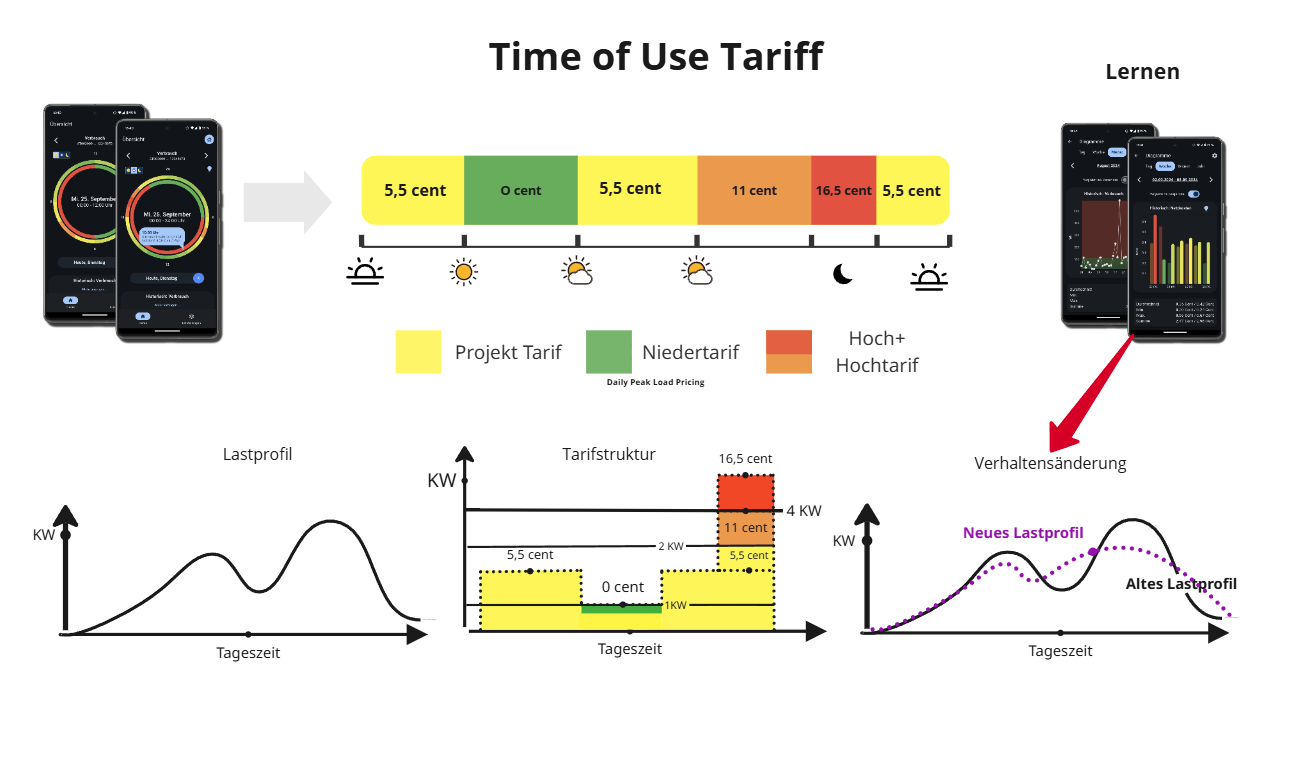
\includegraphics[width=1\linewidth]{paper/figures/ToU.png}
    \caption{Überblick über den Capacity-based-Time-of-Use-Tarif in NOÖ.}
    \label{fig:nooe_tou_design}
\end{figure}



\subsection{Capacity-based Time-of-Use in Netz Oberösterreich}

Der Time-of-Use-Tarif in NOÖ basiert auf täglichen ex-ante Netzsimulationen. Für jede Stunde des Folgetages wird ein Netzzustand klassifiziert: Normalzustand, Überschusssituation oder Engpasssituation. Die Klassifikation wird den Haushalten jeweils am Vortag kommuniziert. Sei \(c_{it}\) der Stromverbrauch von Haushalt \(i\) in einem 15-Minuten-Intervall \(t\).

Im Normalzustand gilt ein konstanter Basistarif:
\begin{equation}
p^{\text{base}} = p^{\text{usage}} + p^{\text{loss}} = 4{,}66 + 0{,}796 \approx 5{,}5 \ \text{ct/kWh}.
\end{equation}

In Überschussperioden wird der Netztarif auf null gesetzt, sofern der Verbrauch einen Schwellenwert erreicht:
\begin{equation}
p_{it} =
\begin{cases}
0, & \text{falls } c_{it} \geq 0{,}25, \\
p^{\text{base}}, & \text{sonst}.
\end{cases}
\end{equation}

In Engpassperioden gilt ein stufenweiser Hochtarif:
\begin{equation}
p_{it} =
\begin{cases}
15{,}7, & \text{falls } c_{it} \geq 1{,}0, \\
10{,}2, & \text{falls } 0{,}5 \leq c_{it} < 1{,}0, \\
p^{\text{base}}, & \text{falls } c_{it} < 0{,}5.
\end{cases}
\end{equation}

Um synchronisierte Lastverschiebungen zu vermeiden, werden Haushalte in Gruppen mit unterschiedlich langen Hochpreisfenstern eingeteilt. Die Zeitfenster umfassen zwei, vier oder sechs Stunden und werden über die Zeit rotiert.

\subsection{Daily Peak Pricing in Linz Netz}

Der Daily-Peak-Pricing-Mechanismus in Linz Netz verwendet die höchste 15-Minuten-Last eines Tages als Bemessungsgrundlage. Fällt die höchste Last in ein definiertes Ausnahmefenster, wird für die Berechnung stattdessen die höchste Last außerhalb dieses Ausnahmefensters herangezogen. Die Ausnahmefenster unterscheiden sich zwischen statischen und dynamischen Gruppen: In der statischen Variante sind die Zeitfenster saisonal vorab festgelegt, während die dynamische Variante auf wetter- beziehungsweise prognosebasierten Zeitfenstern beruht.

\begin{table}[h!]
\centering
\resizebox{\textwidth}{!}{%
\begin{tabular}{llll}
\toprule
\textbf{Saison} & \textbf{Monate} & \textbf{Ausnahmefenster} & \textbf{Dauer} \\ \midrule
Winter & November--Februar & 11:00 bis 13:00 (WT) & 2 Stunden \\
Übergangsperiode & März, April & 10:30 bis 13:30 (WT) & 3 Stunden \\
 & September, Oktober & 11:30 bis 14:30 (ST) & 3 Stunden \\
Sommer & Mai--August & 11:00 bis 15:00 (ST) & 4 Stunden \\
\bottomrule
\end{tabular}%
}
\caption{Geplante saisonale Ausnahmefenster im statischen Daily-Peak-Pricing-Tarif. WT = Winterzeit, ST = Sommerzeit.}
\label{tab:exclusion_periods}
\end{table}

Die Kostenlogik lässt sich vereinfacht wie folgt darstellen:
\[
\text{Gesamtkosten} =
\begin{cases}
    C_{\text{peak}} \times P_{\text{max}} & \text{falls } t \notin \text{Ausnahmefenster}, \\
    C_{\text{peak}} \times P_{\text{next max}} & \text{falls } t \in \text{Ausnahmefenster}.
\end{cases}
\]

Dabei bezeichnet \(C_{\text{peak}}\) den Leistungspreis, \(P_{\text{max}}\) die höchste gemessene 15-Minuten-Leistung eines Tages und \(P_{\text{next max}}\) die höchste Leistung außerhalb des Ausnahmefensters.



\begin{figure}
    \centering
    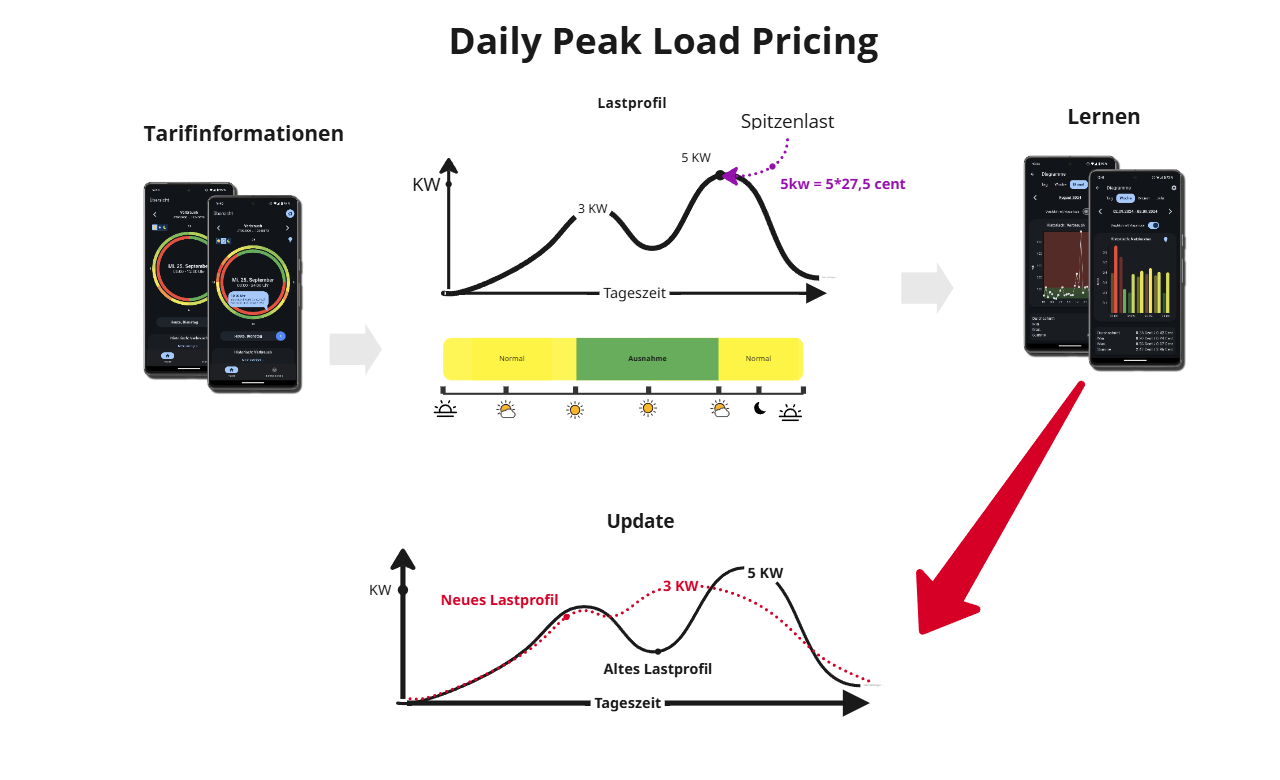
\includegraphics[width=1\linewidth]{paper/figures/CPP.png}
    \caption{Überblick über den Daily-Peak-Pricing-Tarif in LN.}
    \label{fig:ln_cpp_design}
\end{figure}

\subsection{Tarif- und Ausnahmefenster in der Tarifphase}

Tabelle~\ref{tab:tariff_window_hourly_shares} zeigt die Verteilung der Anreize über den Tag. 

\begin{table}[H]
\centering
\scriptsize
\caption{Tarif- und Ausnahmefenster nach Tagesstunde}
\label{tab:tariff_window_hourly_shares}
\begin{flushleft}
\footnotesize Platzhalter -- wird von \texttt{R/03\_tariff\_window\_tables.R} erzeugt, sobald der Report-Pipeline-Lauf vorliegt.
\end{flushleft}
\end{table}


\subsection{Hypothesen}

Das Projekt testet zwei dynamische Netztarifdesigns in parallelen Feldexperimenten. Für LN wird erwartet, dass Haushalte Spitzenlasten außerhalb von Ausnahmefenstern reduzieren und flexible Lasten in Ausnahmefenster verschieben. Für NOÖ wird erwartet, dass Haushalte Verbrauch aus Hochtarifperioden heraus und, soweit möglich, in Niedrigtarifperioden hinein verschieben. In beiden Fällen ist offen, wie stark die Reaktion ausfällt, weil die monetären Anreize relativ klein sind und die Umsetzung Aufmerksamkeit, Verständnis und teilweise technische Flexibilität erfordert.
